\section{Plataforma Codeboard UERJ}

A plataforma Codeboard UERJ é uma ferramenta de ensino de programação que permite a criação de salas de aula virtuais, onde os alunos podem escrever códigos de programação em tempo real. A plataforma foi desenvolvida com base em três princípios fundamentais: colaboração, interatividade e praticidade. Ela foi projetada para ser simples e intuitiva, permitindo que os usuários a utilizem sem a necessidade de treinamento prévio. 

Este capítulo apresenta a plataforma Codeboard UERJ e nele serão abordados os objetivos, funcionalidades e a arquitetura da plataforma.	

\subsection{Objetivos}

O objetivo principal da plataforma Codeboard UERJ é auxiliar no ensino de programação, permitindo que professores criem e gerenciem atividades práticas para seus alunos. A plataforma foi desenvolvida para ser utilizada em disciplinas de programação de computadores, como Algoritmos e Estruturas de Dados, Linguagens de Programação e Paradigmas de Programação.

A motivação para o desenvolvimento da plataforma surgiu durante a pandemia de COVID-19, quando as aulas presenciais foram suspensas e as atividades práticas de programação tiveram que ser adaptadas para o ensino remoto. Ela foi desenvolvida para atender a essa demanda, dando a capacidade aos professores de acompanharem o progresso dos alunos e avaliarem suas atividades práticas em tempo real.


\subsection{Funcionalidades}

Para atingir os objetivos propostos, o desenvolvimento da plataforma foi restrito a um conjunto de funcionalidades essenciais, que são:
Autenticação de usuários, gerenciamento de salas e seus participantes e o quadro de programação em tempo real.

\subsubsection{Autenticação de Usuários}

O sistema de autenticação de usuários é o ponto de partida para o uso da plataforma, permitindo que novos usuários se cadastrem e realizem login para acessar suas funcionalidades. O processo de cadastro ocorre por meio de um formulário que coleta informações básicas, como nome, e-mail e senha. Após a conclusão do cadastro, o usuário está apto a realizar login utilizando o e-mail e a senha fornecidos.

Durante o login, a plataforma valida as credenciais inseridas, verificando se o e-mail e a senha correspondem a uma conta existente. Se os dados forem corretos, o usuário é autenticado e direcionado à página inicial. Caso contrário, uma mensagem de erro é exibida, informando que as credenciais são inválidas. Caso o usuário ainda não tenha uma conta, ele pode acessar a página de cadastro por meio de um link, preencher o formulário e, após o registro, ser redirecionado automaticamente para a tela inicial. Esse processo de autenticação está ilustrado no diagrama de fluxo da Figura \ref{fig:user-auth-flow}, com as telas de login e cadastro exibidas nas Figuras \ref{fig:login-page} e \ref{fig:signup-page}, respectivamente.

\begin{figure}[H]
    \centering
    \includegraphics[width=1\textwidth]{diagrams/user-auth-flow.png}
    \caption{Diagrama do fluxo de autenticação de usuários.}
    \label{fig:user-auth-flow}
\end{figure}

\begin{figure}[H]
    \centering
    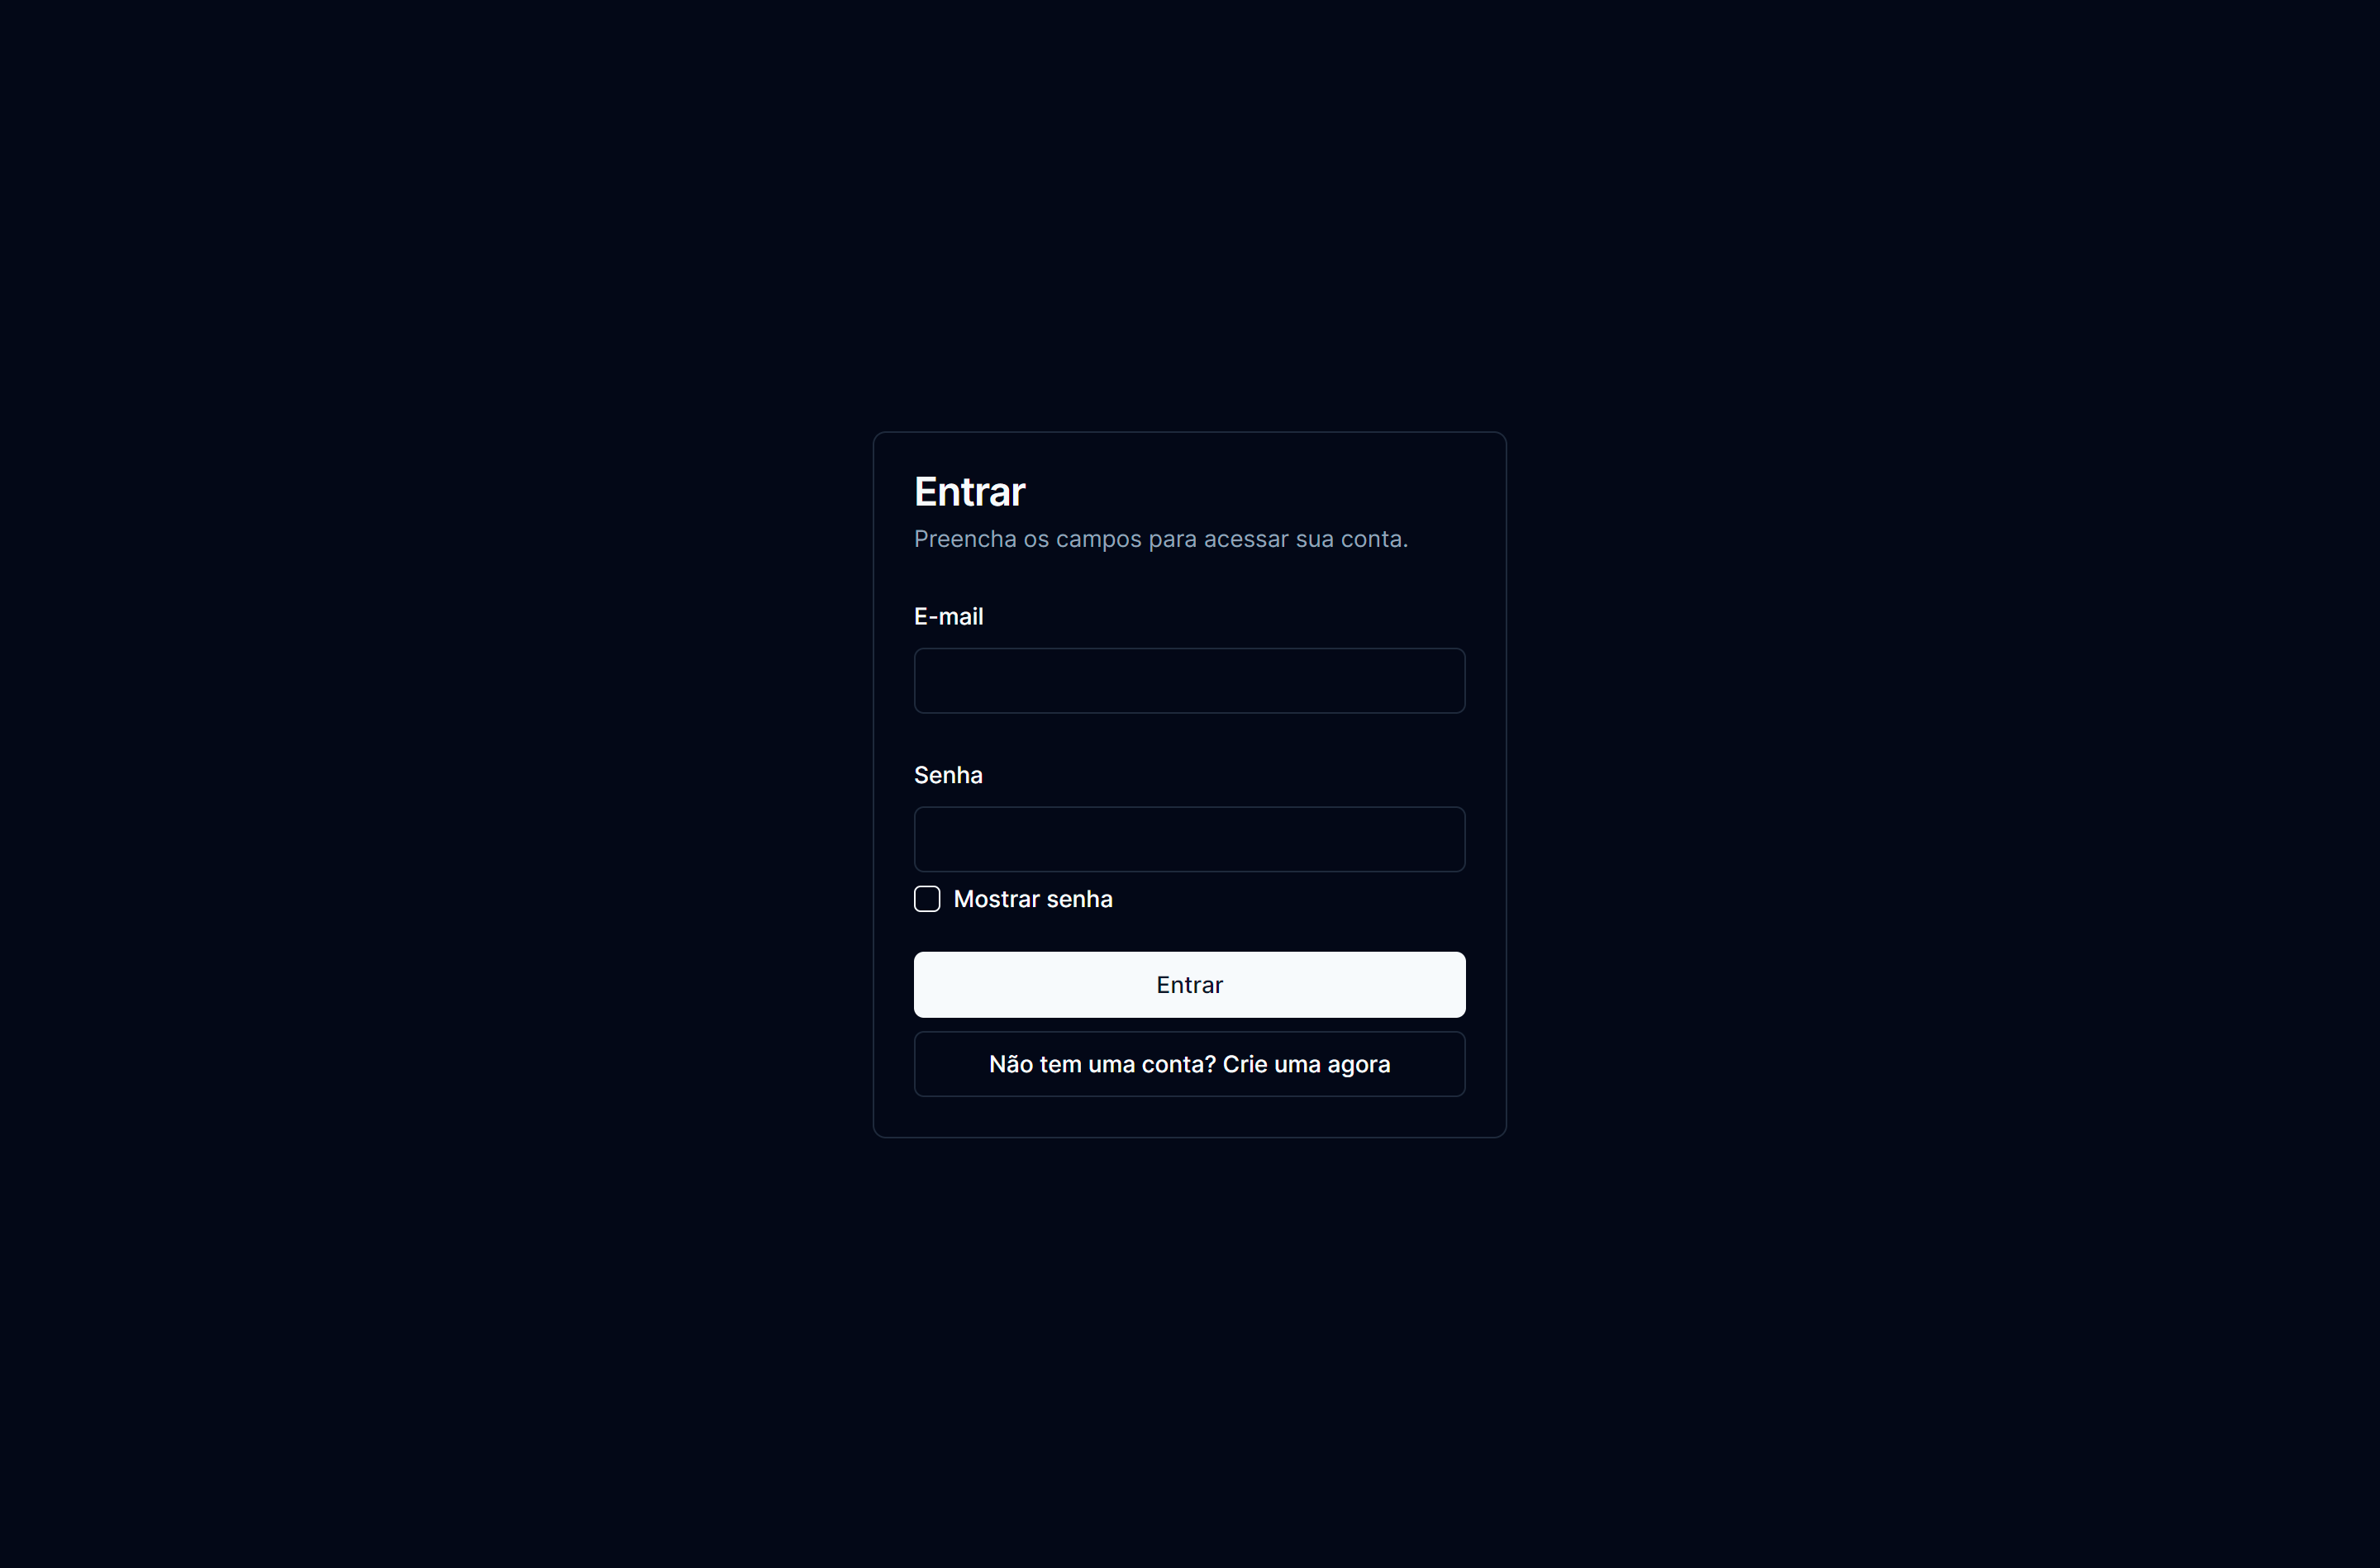
\includegraphics[width=0.8\textwidth]{assets/codeboard/login-page.png}
    \caption{Página de login da plataforma Codeboard UERJ.}
    \label{fig:login-page}
\end{figure}

\begin{figure}[H]
    \centering
    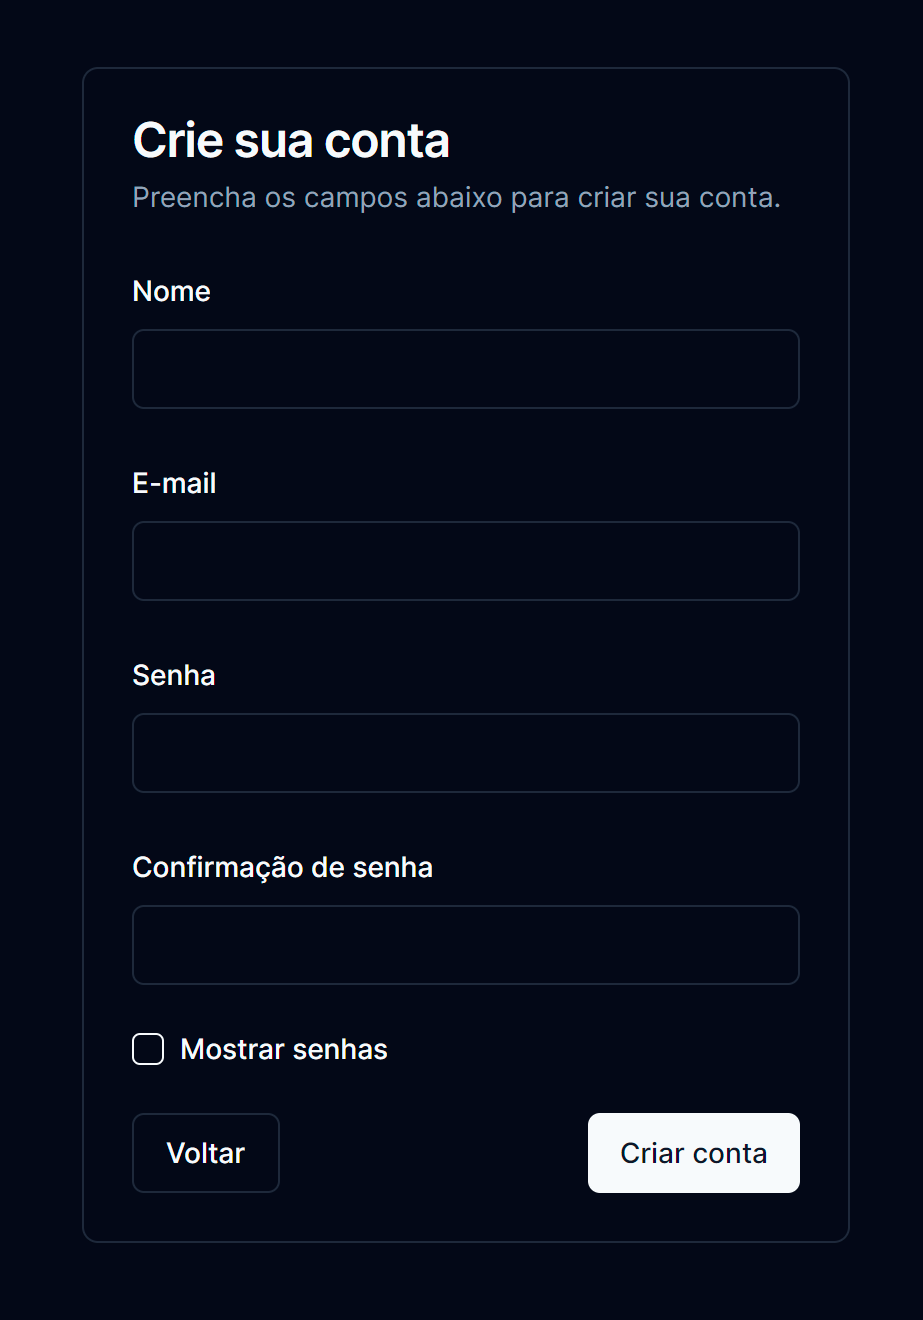
\includegraphics[width=0.8\textwidth]{assets/codeboard/signup-page.png}
    \caption{Página de cadastro da plataforma Codeboard UERJ.}
    \label{fig:signup-page}
\end{figure}

Durante o processo de autenticação, a plataforma utiliza tokens para manter a sessão do usuário ativa. O token é gerado no servidor e enviado ao cliente, sendo armazenado no navegador por meio de cookies. Esse token é então utilizado em todas as requisições subsequentes feitas ao servidor, garantindo que o usuário permaneça autenticado enquanto navega pelas diversas páginas da plataforma.

\subsubsection{Gerenciamento de Salas}

A funcionalidade de gerenciamento de salas, ilustrada na Figura \ref{fig:rooms-page}, constitui a página inicial da plataforma. Nessa página, as salas são apresentadas em uma lista, onde cada sala é representada por um cartão que exibe o nome, a descrição e o número de participantes. O usuário pode acessar uma sala ao clicar no respectivo cartão, sendo então redirecionado para a tela da sala.

\begin{figure}[H]
    \centering
    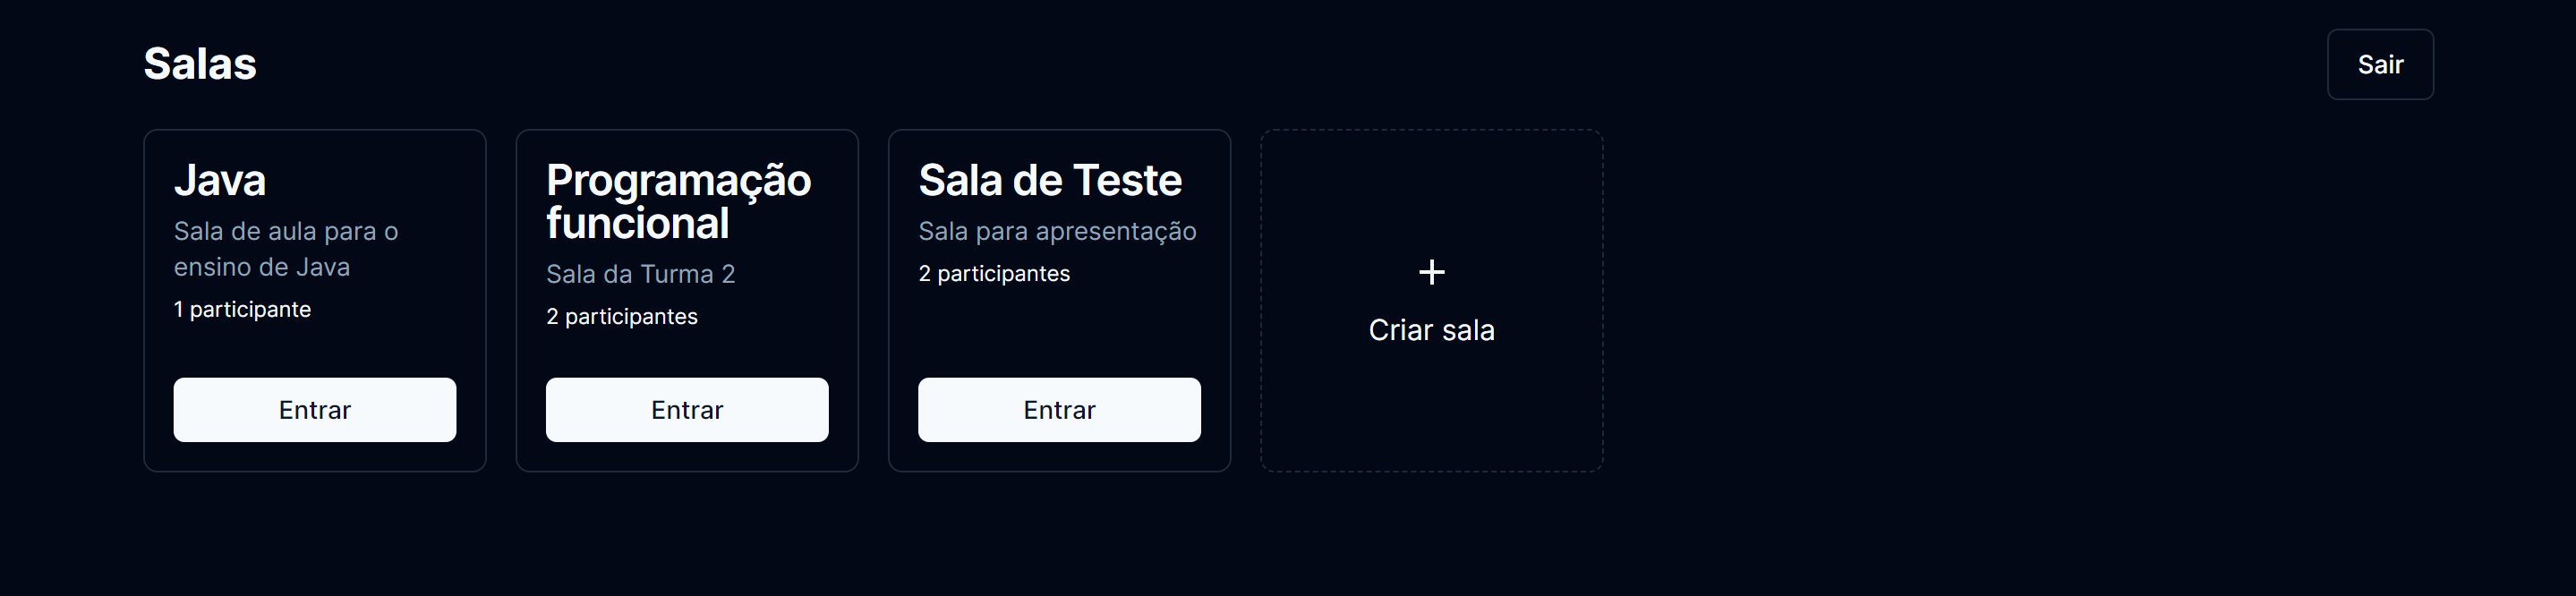
\includegraphics[width=1\textwidth]{assets/codeboard/rooms-page.png}
    \caption{Página de listagem de salas da plataforma Codeboard UERJ.}
    \label{fig:rooms-page}
\end{figure}


Além disso, o usuário pode criar uma nova sala diretamente na tela inicial, utilizando o botão de criação de sala. Ao clicar no botão, o usuário é redirecionado para a página de criação de sala, mostrada na Figura \ref{fig:create-room-page}. Nessa página, é possível inserir o nome e a descrição da sala para concluir a criação

\begin{figure}[H]
    \centering
    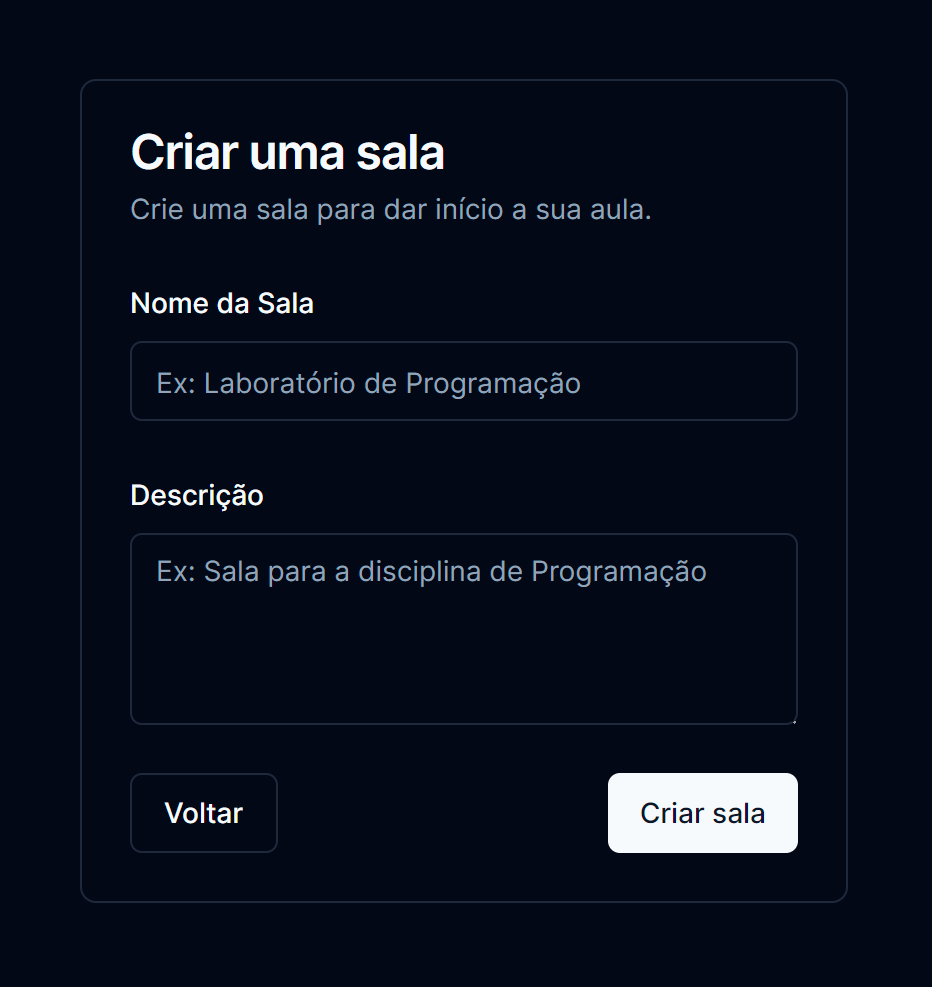
\includegraphics[width=0.7\textwidth]{assets/codeboard/create-room-page.png}
    \caption{Página de criação de sala da plataforma Codeboard UERJ.}
    \label{fig:create-room-page}
\end{figure}

Após a criação, o usuário é redirecionado para a tela da sala. Para adicionar novos membros, basta clicar no botão de adição de participantes, identificado por um ícone de usuário, conforme mostrado na Figura \ref{fig:add-member-modal}. Uma nova tela será exibida com um campo para inserção do e-mail do aluno que se deseja adicionar à sala. Após a inclusão, o aluno torna-se membro da sala e pode acessá-la.

\begin{figure}[H]
    \centering
    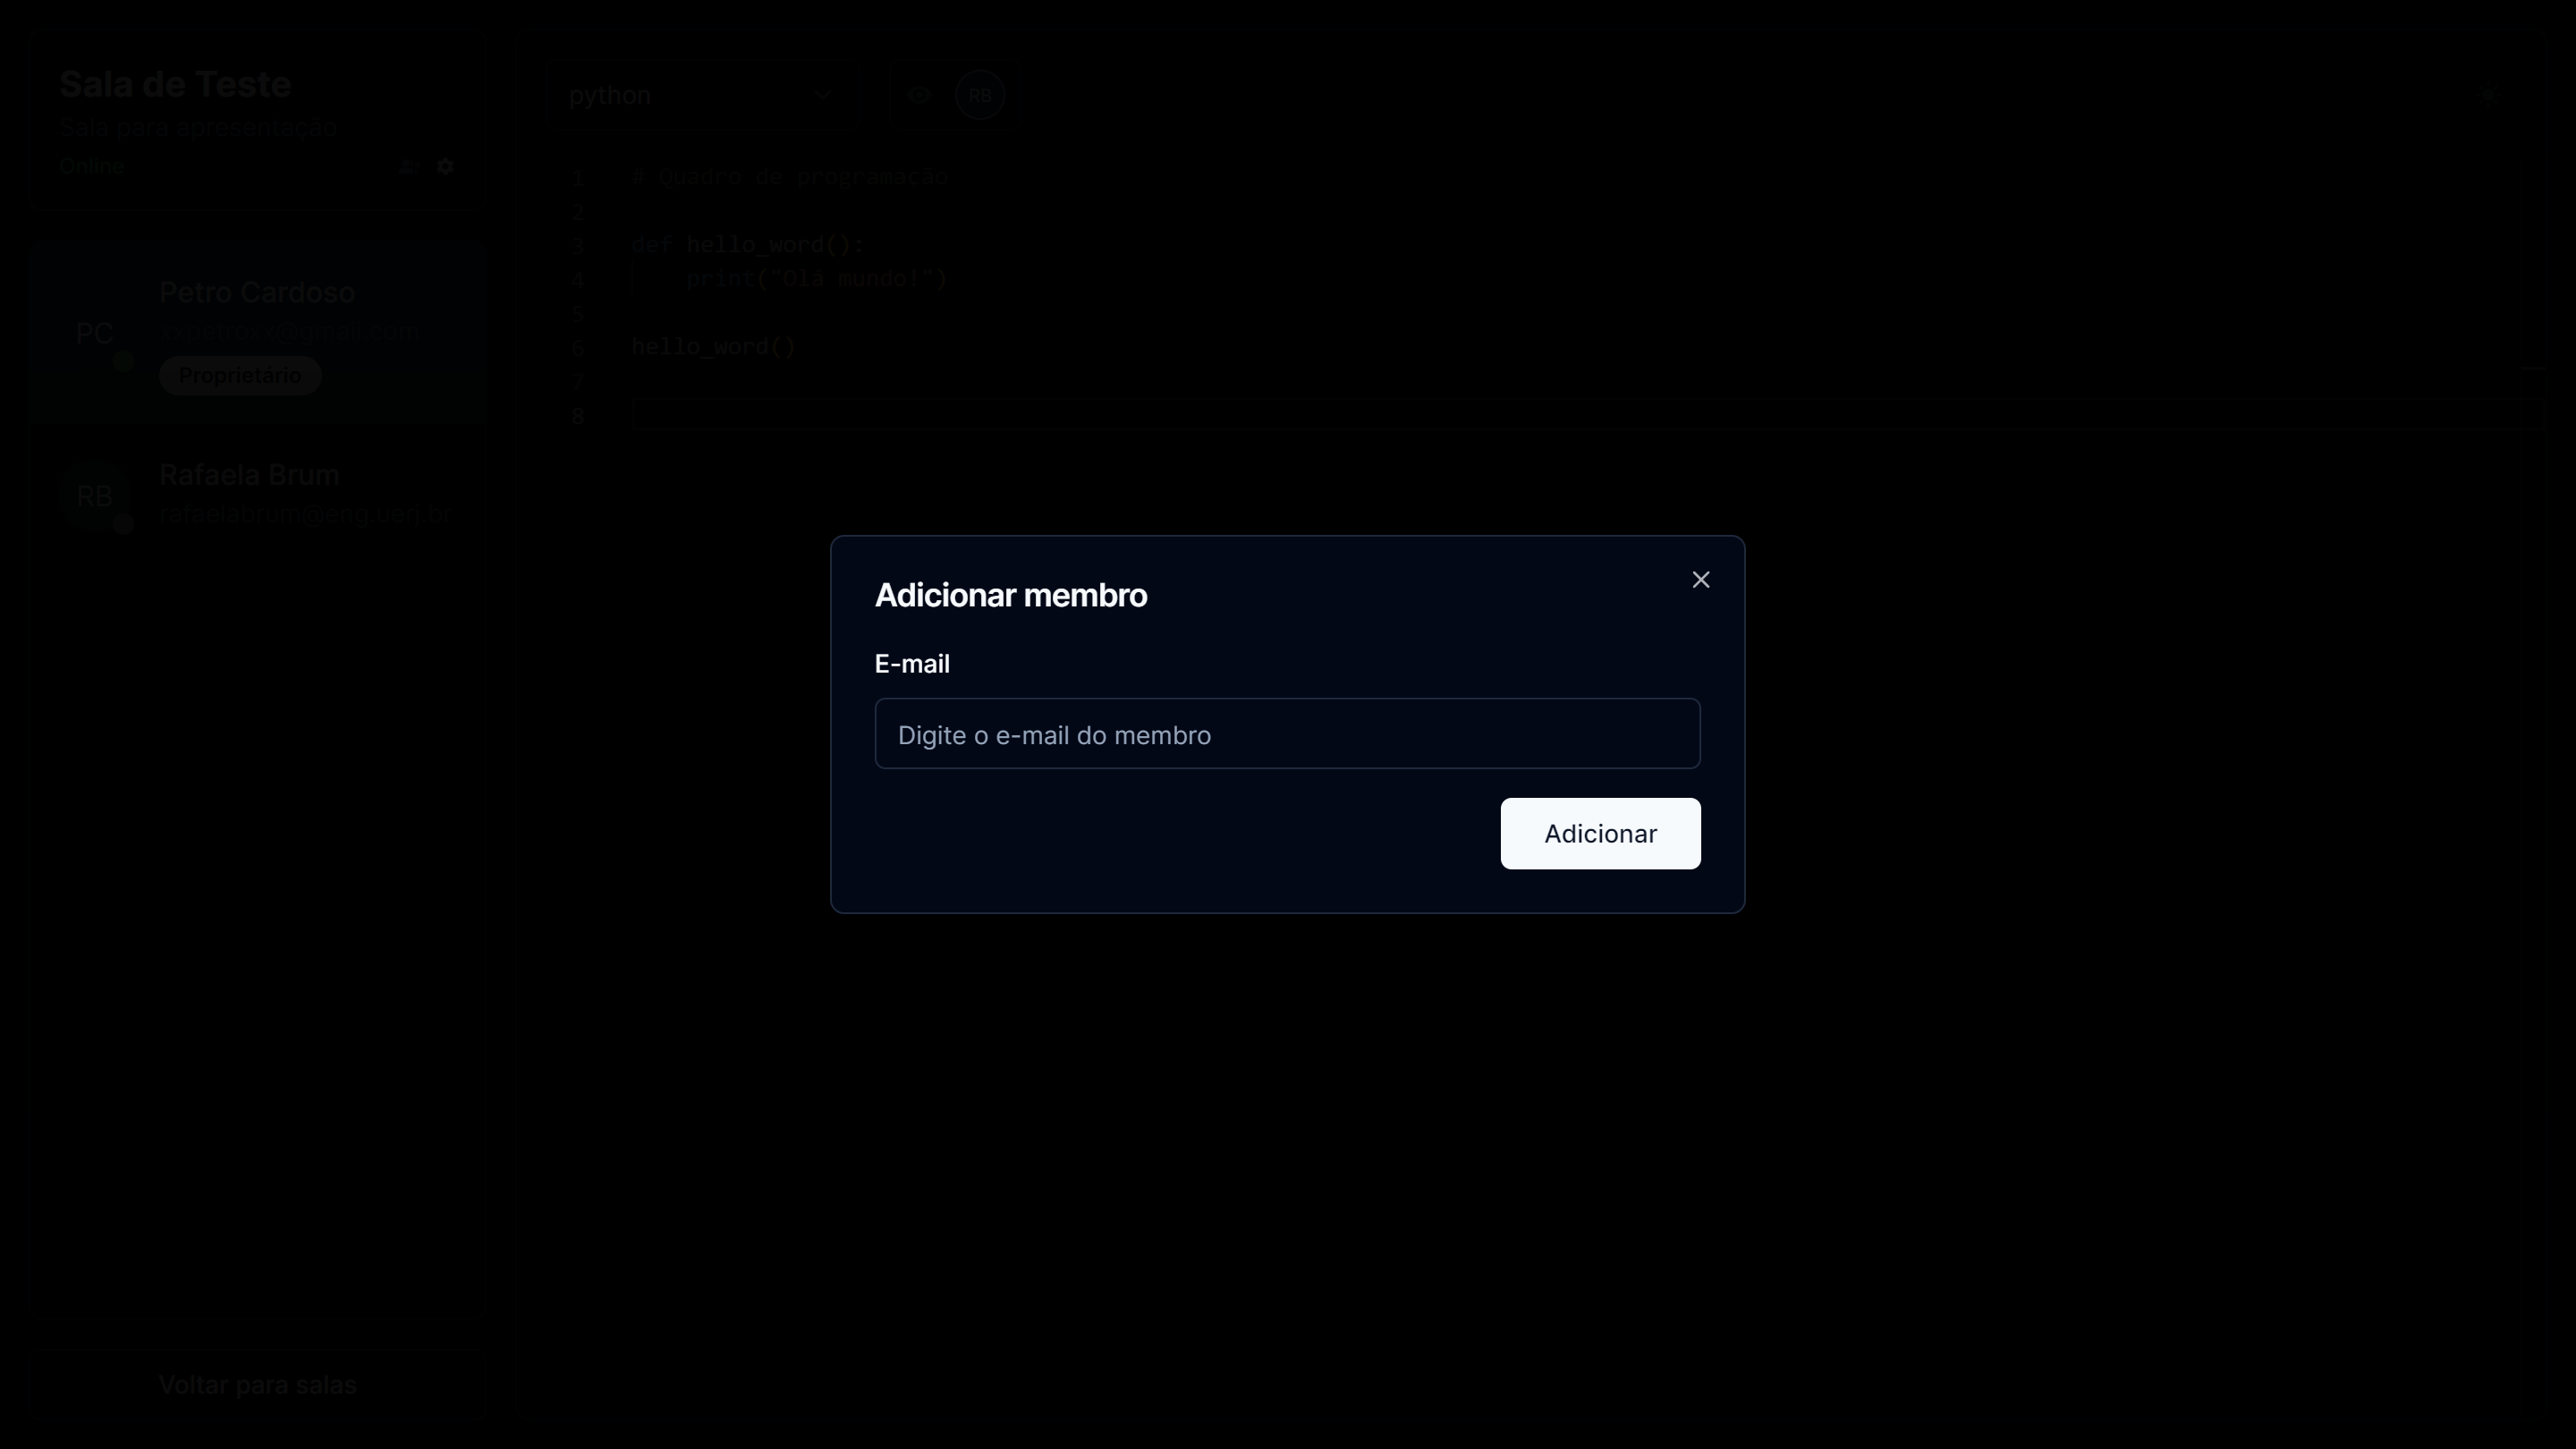
\includegraphics[width=0.8\textwidth]{assets/codeboard/add-member-modal.png}
    \caption{Tela de adição de alunos à sala da plataforma Codeboard UERJ.}
    \label{fig:add-member-modal}
\end{figure}


O fluxo descrito do gerenciamento de salas está representado no diagrama da Figura \ref{fig:user-room-flow}.


\begin{figure}[H]
    \centering
    \includegraphics[width=0.8\textwidth]{diagrams/user-room-flow.png}
    \caption{Diagrama do fluxo de gerenciamento de salas.}
    \label{fig:user-room-flow}
\end{figure}


\subsubsection{Quadro de Programação em Tempo Real}

% TODO: TO AQUIII
 
A funcionalidade de quadro de programação em tempo real é a principal funcionalidade da plataforma. Ela permite que os alunos escrevam códigos de programação diretamente no navegador, sem a necessidade de instalar um ambiente de desenvolvimento integrado (IDE).

Para acessar o quadro de programação, o usuário deve acessar a sala desejada. A plataforma exibe uma tela dividida em dois módulos, o módulo lateral de seleção de usuário e o módulo central de edição de código.

\begin{figure}[H]
    \centering
    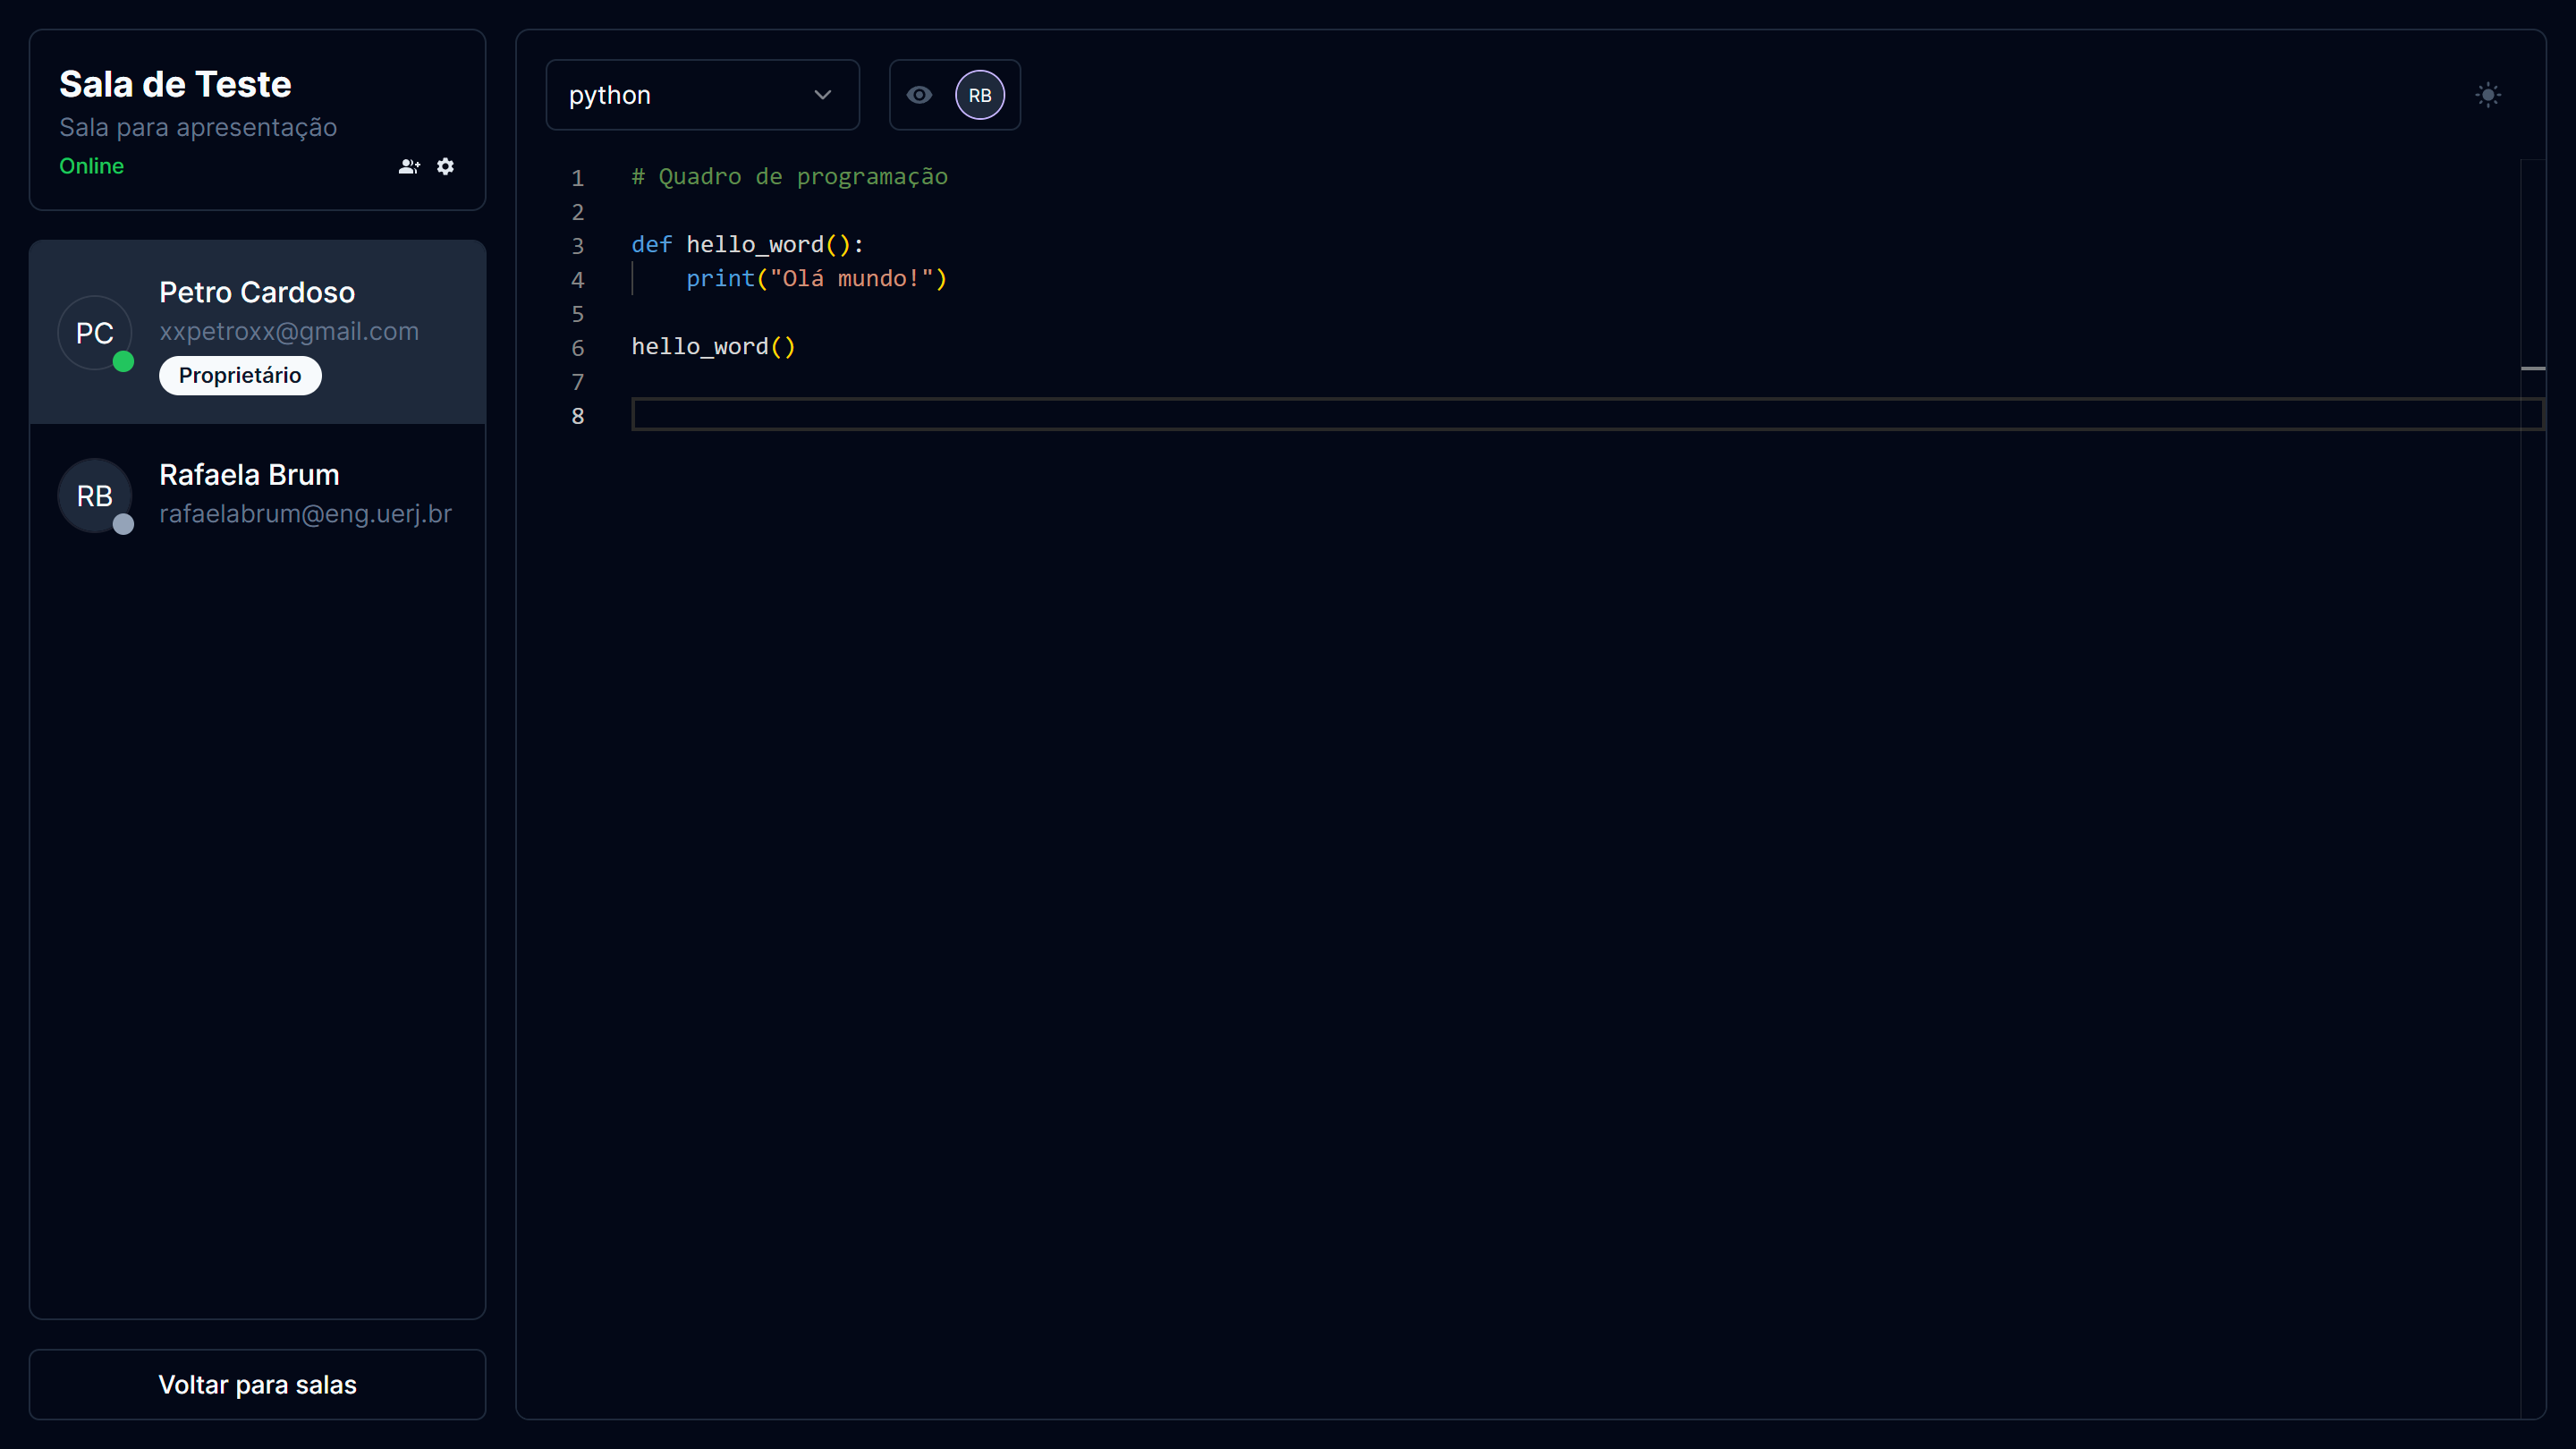
\includegraphics[width=0.8\textwidth]{assets/codeboard/room-details-page.png}
    \caption{Página da sala de programação da plataforma Codeboard UERJ.}
    \label{fig:room-details-page}
\end{figure}


Como mostra a figura \ref{fig:room-details-page}, o módulo lateral exibe a lista de participantes da sala. Para cada membro listado, é exibido o nome, a foto de perfil e indicadores para caso ele esteja online ou esteja editando o seu próprio código. O usuário pode selecionar outro membro da sala na lista lateral para visualizar e interagir com o código dele.

Caso o usuário já esteja com si mesmo selecionado, ele poderá editar o próprio código, trocar de linguagem de programação e visualizar quem está visualizando seu código. O código é salvo automaticamente a cada edição realizada pelo usuário.

Acima do módulo lateral, a plataforma exibe o nome da sala e sua descrição. Caso o usuário seja o dono da sala, também serão exibidos os botões de adição de participantes e de configuração da sala. O botão de adição de participantes permite que o usuário adicione novos participantes à sala, enquanto o botão de configuração permite que o usuário edite o nome e a descrição da sala.

\begin{figure}[H]
    \centering
    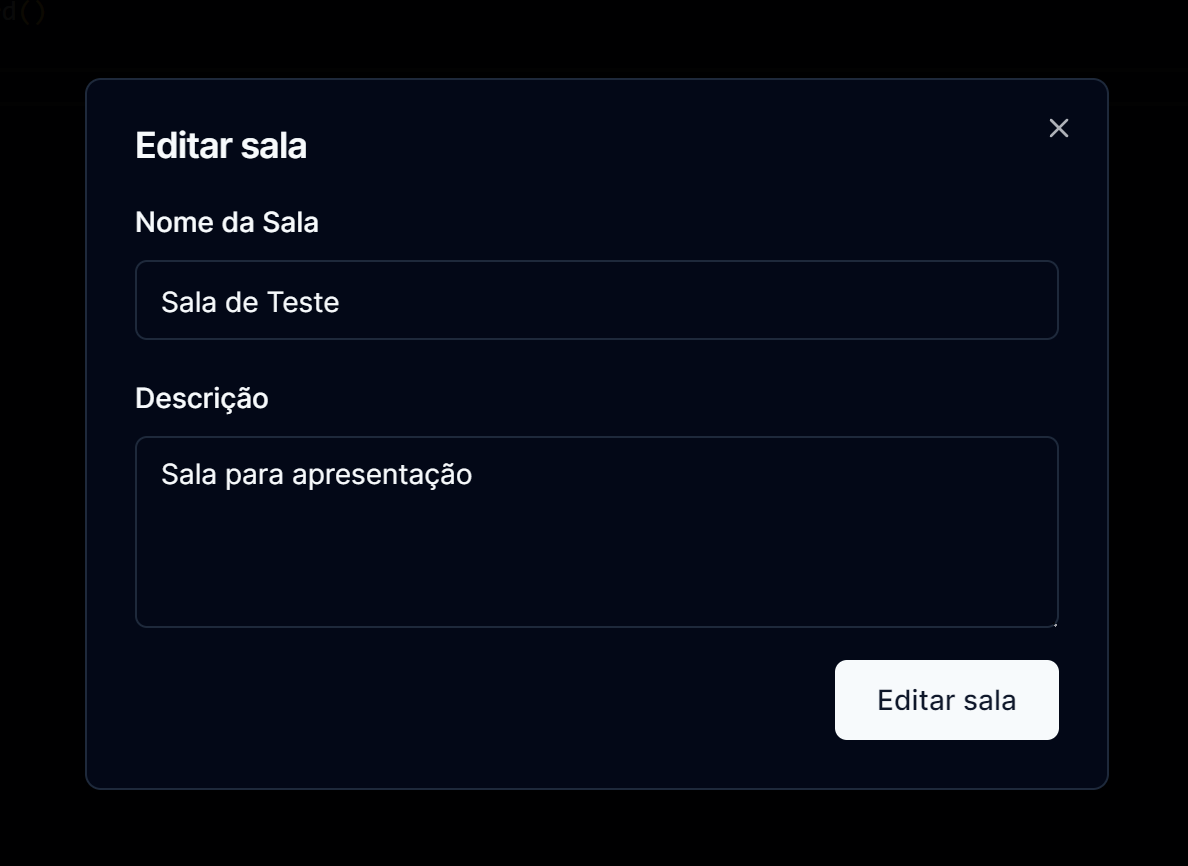
\includegraphics[width=0.8\textwidth]{assets/codeboard/edit-room-modal.png}
    \caption{Modal de configuração de sala da plataforma Codeboard UERJ.}
    \label{fig:edit-room-modal}
\end{figure}


Abaixo do módulo lateral, a plataforma exibe um botão de saída da sala. Ao clicar neste botão, o usuário é redirecionado para a tela de listagem de salas, onde ele pode acessar outras salas ou criar uma nova sala.

O módulo central exibe o editor de código. Este editor suporta as funcionalidades básicas de um IDE, como coloração de sintaxe, auto-completar e formatação de código. Durante a visualização do código de outro usuário, o usuário pode somente fazer marcações que são exibidas em tempo real para o outros usuários presentes no quadro.

\begin{figure}[H]
    \centering
    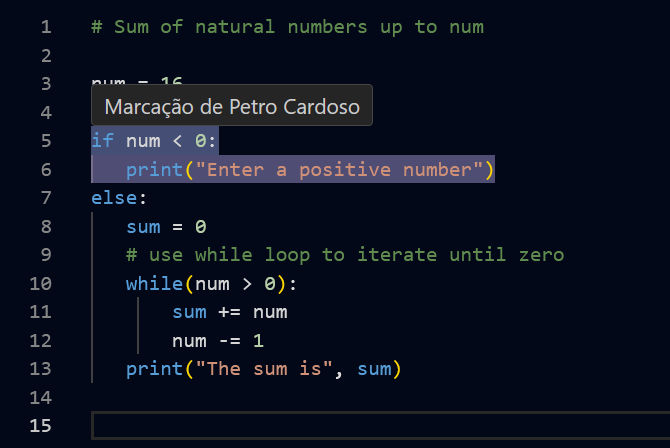
\includegraphics[width=0.8\textwidth]{assets/codeboard/code-editor-user-highlight.png}
    \caption{Marcação de código na plataforma Codeboard UERJ.}
    \label{fig:code-editor-user-highlight}
\end{figure}

Na parte superior do editor, o usuário pode selecionar a linguagem de programação desejada. A plataforma suporta as linguagens de programação mais utilizadas, como C, C++, Java, Python, JavaScript, entre outras. A seleção da linguagem de programação altera a coloração de sintaxe do editor, facilitando a escrita e a leitura do código.

\begin{figure}[H]
    \centering
    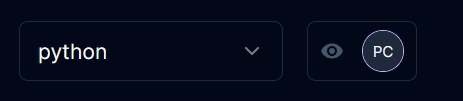
\includegraphics[width=0.8\textwidth]{assets/codeboard/code-editor-toolbar.png}
    \caption{Barra de ferramentas do editor de código da plataforma Codeboard UERJ.}
    \label{fig:code-editor-toolbar}
\end{figure}

Ao lado da seleção de linguagem, o usuário pode visualizar quem está visualizando o seu código no momento. A plataforma exibe uma lista horizontal com estes visualizadores, permitindo que ele saiba quem está acompanhando o seu progresso.


\subsubsection{Regras de Negócio}

Existem algumas regras de negócio que devem ser seguidas para garantir o bom funcionamento da plataforma. Estas regras são implementadas no backend da plataforma e são responsáveis por validar os dados dos usuários e das salas, bem como garantir a segurança e a integridade dos dados.

\paragraph{Autenticação}

\begin{itemize}
    \item \textbf{Cadastro de Usuários}: A plataforma deve fornecer um mecanismo de cadastro de usuários que permita aos usuários se registrarem na plataforma. Para isso, é necessário solicitar os dados dos usuários, como nome, e-mail e senha, e armazená-los de forma segura e protegida no banco de dados.
    \item \textbf{Validação de Dados}: A plataforma deve garantir que os dados dos usuários sejam válidos e consistentes. Para isso, é necessário validar os dados dos usuários durante o processo de cadastro e login e garantir que os dados sejam consistentes e íntegros.
    \item \textbf{Proteção de Dados}: A plataforma deve garantir que os dados dos usuários sejam protegidos e seguros. Para isso, é necessário armazenar os dados dos usuários de forma segura e protegida, utilizando técnicas de criptografia e hash de senhas.
    \item \textbf{Login de Usuários}: A plataforma deve garantir que somente usuários cadastrados possam fazer login. Para isso, é necessário verificar se o e-mail e a senha informados são válidos durante o processo de login e gerar um token de autenticação para manter o usuário autenticado.
    \item \textbf{Gerenciamento de Sessões}: A plataforma deve garantir que as sessões dos usuários sejam gerenciadas de forma segura e eficiente. Para isso, é necessário gerar tokens de autenticação para manter os usuários autenticados e garantir que as sessões sejam encerradas após um período de inatividade.
    \item \textbf{Restrição de Acesso}: A plataforma deve garantir que somente usuários autenticados tenham acesso às funcionalidades da plataforma. Para isso, é necessário verificar se o usuário está autenticado antes de permitir o acesso às funcionalidades.
\end{itemize}

\paragraph{Gerenciamento de Salas}

\begin{itemize}
    \item \textbf{Criação de Salas}: A plataforma deve fornecer um mecanismo de criação de salas que permita aos usuários criarem novas salas. Para isso, é necessário solicitar os dados das salas, como nome e descrição, e armazená-los de forma segura e protegida no banco de dados.
    \item \textbf{Validação de Dados}: A plataforma deve garantir que os dados das salas sejam válidos e consistentes. Para isso, é necessário validar os dados das salas durante o processo de criação e edição e garantir que os dados sejam consistentes e íntegros.
    \item \textbf{Restrição de Acesso}: A plataforma deve garantir que somente participantes da sala tenham acesso à ela. Para isso, é necessário verificar se o usuário é dono ou membro da sala antes de permitir o acesso à sala.
    \item \textbf{Gerenciamento de Participantes}: A plataforma deve fornecer um mecanismo de adição e remoção de participantes que permita aos usuários gerenciarem os participantes das salas. Para isso, é necessário verificar se o usuário é dono da sala antes de permitir a adição ou remoção de participantes.
    \item \textbf{Restrição de Edição}: A plataforma deve garantir que somente o dono da sala possa editar os dados da sala. Para isso, é necessário verificar se o usuário é dono da sala antes de permitir a edição dos dados da sala.
\end{itemize}

\paragraph{Quadro de Programação}

\begin{itemize}
    \item \textbf{Editor em Tempo Real}: A plataforma deve fornecer um mecanismo de edição de código em tempo real que permita aos usuários escrever códigos de programação diretamente no navegador. Para isso, é necessário implementar um editor de código que suporte as funcionalidades básicas de um IDE, como coloração de sintaxe, auto-completar e formatação de código.
    \item \textbf{Restrição de Escrita}: A plataforma deve garantir que não haja conflitos de escrita durante a edição do código em tempo real. Para isso, é necessário implementar um mecanismo de bloqueio de escrita que permita que somente o proprietário do código possa editá-lo.
    \item \textbf{Marcação de Código}: A plataforma deve fornecer um mecanismo de marcação de texto que permita aos usuários visualizarem e interagirem com o código de outros usuários. Para isso, é necessário implementar um mecanismo de marcação que exiba as alterações em tempo real para os outros usuários presentes no quadro.
    \item \textbf{Seleção de Linguagem}: A plataforma deve fornecer um mecanismo de seleção de linguagem que permita aos usuários escolher a linguagem de programação desejada. Para isso, é necessário implementar um seletor de linguagem que altere a coloração de sintaxe do editor de código.
    \item \textbf{Visualização de Usuários}: A plataforma deve fornecer um mecanismo de visualização de usuários que permita aos usuários saber quem está visualizando o seu código. Para isso, é necessário implementar uma lista de visualizadores que exiba os usuários presentes no quadro.
\end{itemize}

\paragraph{Lista de Participantes}

\begin{itemize}
    \item \textbf{Visualização de Participantes}: A plataforma deve fornecer um mecanismo de visualização de participantes que permita aos usuários saber quem está presente na sala. Para isso, é necessário implementar uma lista de participantes que exiba os usuários presentes na sala.
    \item \textbf{Indicadores de Presença}: A plataforma deve fornecer um mecanismo de indicação de presença que permita aos usuários saber quem está online e quem está editando o código. Para isso, é necessário implementar indicadores de presença que exibam se o usuário está online e se está editando o código.
    \item \textbf{Seleção de Participantes}: A plataforma deve fornecer um mecanismo de seleção de participantes que permita aos usuários visualizarem e interagirem com o código de outros participantes. Para isso, é necessário implementar um seletor de participantes que permita selecionar o participante desejado.
\end{itemize}


\subsection{Arquitetura da Plataforma}
% Revisado

Nesta seção, será apresentada a arquitetura da plataforma Codeboard UERJ. A plataforma é estruturada em três camadas principais: o backend, o banco de dados e o frontend. Cada uma dessas camadas desempenha um papel específico na plataforma, sendo responsável pelas regras de negócio, o armazenamento de dados e a interface com o usuário, respectivamente.

\subsubsection{Backend}
% Revisado

O backend da plataforma é responsável pela implementação das regras de negócio da aplicação. Ele é composto por um servidor NodeJS que utiliza dois métodos de comunicação: REST API e WebSockets. A REST API é usada para comunicação assíncrona entre o cliente e o servidor, enquanto os WebSockets são utilizados para permitir a comunicação em tempo real entre os usuários.

\begin{figure}[H]
    \centering
    \includegraphics[width=0.75\textwidth]{diagrams/backend-architecture.png}
    \caption{Arquitetura do backend da plataforma Codeboard UERJ.}
    \label{fig:backend-architecture}
\end{figure}

Conforme a arquitetura do backend ilustrada na Figura \ref{fig:backend-architecture}, a comunicação entre o cliente e o servidor ocorre através de duas interfaces principais: REST API e WebSockets. A REST API fornece um conjunto de rotas que permitem ao cliente acessar funcionalidades da plataforma, como autenticação de usuários, gerenciamento de salas e edição de código. Os WebSockets, por sua vez, são utilizados para viabilizar a comunicação em tempo real entre os usuários, possibilitando a edição colaborativa de código.


\subsubsection{Banco de Dados NoSQL}
% Revisado

A plataforma utiliza o MongoDB como banco de dados, um sistema NoSQL orientado a documentos. O MongoDB foi escolhido por sua flexibilidade, capacidade de escalabilidade horizontal e eficiência no armazenamento de grandes volumes de dados. Além disso, sua integração simples com o NodeJS o torna uma escolha natural para a plataforma Codeboard UERJ.

O banco de dados é organizado em duas coleções principais: a coleção de usuários e a coleção de salas. A coleção de usuários armazena informações dos usuários cadastrados na plataforma, como nome, e-mail e senha. Já a coleção de salas guarda os dados das salas criadas pelos usuários, incluindo nome, descrição e participantes.

\begin{figure}[H]
    \centering
    \includegraphics[width=0.7\textwidth]{diagrams/database-schema.png}
    \caption{Esquema do banco de dados da plataforma Codeboard UERJ.}
    \label{fig:database-schema}
\end{figure}

Conforme o esquema do banco de dados ilustrado na Figura \ref{fig:database-schema}, a coleção "User", responsável por armazenar os dados dos usuários, inclui os seguintes campos:

\begin{table}[H]
    \centering
    \renewcommand{\arraystretch}{1.3} 
    \begin{tabular}{|c|c|c|c|}
        \hline
        \textbf{Campo} & \textbf{Descrição}             & \textbf{Tipo} & \textbf{Obrigatório} \\
        \hline
        \_id           & Identificador único do usuário & ObjectId      & Sim                  \\
        \hline
        name           & Nome do usuário                & String        & Sim                  \\
        \hline
        email          & E-mail do usuário              & String        & Sim                  \\
        \hline
        password       & Hash da senha do usuário       & String        & Sim                  \\
        \hline
        createdAt      & Data de criação do usuário     & Date          & Sim                  \\
        \hline
    \end{tabular}
    \caption{Campos da coleção "User" do banco de dados da plataforma Codeboard UERJ.}
    \label{tab:user-collection-fields}
\end{table}

É importante destacar que a coleção de usuários possui um campo "password" que armazena o hash da senha do usuário. Essa prática é adotada por motivos de segurança, garantindo que a senha do usuário não seja armazenada em texto puro no banco de dados, o que poderia expor as informações dos usuários em caso de vazamento de dados.

A coleção "Room", responsável por armazenar os dados das salas, contém os seguintes campos:

\begin{table}[H]
    \centering
    \renewcommand{\arraystretch}{1.3} 
    \begin{tabular}{|c|c|c|c|}
        \hline
        \textbf{Campo} & \textbf{Descrição}             & \textbf{Tipo}   & \textbf{Obrigatório} \\
        \hline
        \_id           & Identificador único da sala    & ObjectId        & Sim                  \\
        \hline
        name           & Nome da sala                   & String          & Sim                  \\
        \hline
        description    & Descrição da sala              & String          & Não                  \\
        \hline
        owner          & Identificador do dono da sala  & ObjectId        & Sim                  \\
        \hline
        members        & Lista de participantes da sala & Array<ObjectId> & Não                  \\
        \hline
        createdAt      & Data de criação da sala        & Date            & Sim                  \\
        \hline
    \end{tabular}
    \caption{Campos da coleção "Room" do banco de dados da plataforma Codeboard UERJ.}
    \label{tab:room-collection-fields}
\end{table}


Podemos observar que a coleção de salas possui os campos "owner" e "members" que armazenam os identificadores do dono e dos participantes da sala, respectivamente. Estes campos são utilizados para estabelecer a relação entre os usuários e as salas.

A coleção "Board", responsável por armazenar os dados dos quadros de programação, contém os seguintes campos:

\begin{table}[H]
    \centering
    \renewcommand{\arraystretch}{1.3} 
    \begin{tabular}{|c|c|c|c|}
        \hline
        \textbf{Campo} & \textbf{Descrição}             & \textbf{Tipo} & \textbf{Obrigatório} \\
        \hline
        \_id           & Identificador único do quadro  & ObjectId      & Sim                  \\
        \hline
        user         & Identificador do usuário dono do quadro & ObjectId      & Sim                  \\
        \hline
        room         & Identificador da sala do quadro & ObjectId      & Sim                  \\
        \hline
        language       & Linguagem de programação       & String        & Sim                  \\
        \hline
        content           & Código de programação          & String        & Sim                  \\
        \hline
        updatedAt      & Data da última atualização      & Date          & Não                  \\
        \hline
        createdAt      & Data de criação      & Date          & Sim                  \\
        \hline
    \end{tabular}
    \caption{Campos da coleção "Board" do banco de dados da plataforma Codeboard UERJ.}
    \label{tab:board-collection-fields}
\end{table}

A coleção de "Board" possui os campos "user" e "room" que armazenam os identificadores do usuário dono do quadro e da sala do quadro, respectivamente. Esses campos são utilizados para estabelecer a relação entre os usuários, as salas e os quadros de programação.


Embora o banco de dados seja NoSQL, a plataforma Codeboard UERJ adota um esquema de dados bem definido para assegurar a consistência e a integridade das informações. Esse esquema é estabelecido no backend da plataforma com o auxílio do pacote "mongoose", que simplifica a modelagem dos dados e a interação com o banco de dados MongoDB.

\subsubsection{Comunicação Síncrona via REST API}
% Revisado

A REST API é formada por um conjunto de rotas que possibilitam ao cliente acessar as funcionalidades da plataforma. Essas rotas são implementadas com o framework ExpressJS, que facilita a criação de rotas e middlewares em aplicações NodeJS.

Na REST API, existem três tipos principais de rotas: de autenticação, de usuários e de salas. As rotas de autenticação são responsáveis pela criação e autenticação de usuários, enquanto as rotas de usuários permitem o acesso e a atualização dos dados dos usuários. Já as rotas de salas são utilizadas para criar, acessar e gerenciar as salas.

\begin{table}[H]
    \centering
    \renewcommand{\arraystretch}{1.3} 
    \begin{tabular}{|c|c|c|c|}
        \hline
        \textbf{Método} & \textbf{Rota}                  & \textbf{Descrição}            & \textbf{Autenticação} \\
        \hline
        GET             & /api/health                    & Verifica o status do servidor & Não                   \\
        \hline
        POST            & /api/auth/signup               & Cadastra um novo usuário      & Não                   \\
        POST            & /api/auth/login                & Autentica um usuário          & Não                   \\
        \hline
        GET             & /api/user                      & Retorna os dados do usuário   & Sim                   \\
        PUT             & /api/user                      & Edita os dados do usuário     & Sim                   \\
        \hline
        GET             & /api/rooms                     & Lista todas as salas          & Sim                   \\
        POST            & /api/rooms                     & Cria uma nova sala            & Sim                   \\
        GET             & /api/rooms/:id                 & Retorna uma sala específica   & Sim                   \\
        PUT             & /api/rooms/:id                 & Edita uma sala específica     & Sim                   \\
        POST            & /api/rooms/:id/members         & Adiciona um membro à sala     & Sim                   \\
        DELETE          & /api/rooms/:id/members/:userId & Remove um membro da sala      & Sim                   \\
        \hline
    \end{tabular}
    \caption{Rotas da REST API da plataforma Codeboard UERJ.}
    \label{tab:rest-api-routes}
\end{table}


\subsubsection{Sistema de Autenticação}
% Revisado

As rotas descritas na tabela \ref{tab:rest-api-routes} que requerem autenticação, são protegidas por um middleware que verifica se o usuário está autenticado antes de permitir o acesso. A autenticação do usuário na plataforma é realizada através de um token, que é gerado no servidor e enviado ao cliente após o login. 

O token de autenticação é gerado utilizando o pacote "jsonwebtoken", que implementa o padrão JWT (JSON Web Token). A escolha do JWT como mecanismo de autenticação foi motivada pela necessidade de suportar a infraestrutura horizontal da plataforma, que facilita a escalabilidade e a distribuição dos servidores. Como o JWT é um mecanismo stateless, não é necessário armazenar o estado da sessão no servidor. Isso o torna ideal para aplicações distribuídas e escaláveis, pois o estado da sessão é armazenado no próprio token, que é enviado ao cliente.

O token é criado com base no ID do usuário e uma chave secreta, que é mantida nos servidores. Esse token é assinado com a chave secreta e enviado ao cliente, onde é armazenado no navegador por meio de cookies. A cada requisição feita ao servidor, o token é utilizado para autenticar o usuário, garantindo sua autenticidade em todas as páginas da plataforma.

O token de autenticação tem um tempo de expiração configurado no servidor. Após esse período, o token é invalidado, e o usuário é automaticamente desconectado da plataforma.

\subsubsection{Banco de Dados Chave-Valor}
% Revisado OK

A plataforma Codeboard UERJ utiliza o Redis, um banco de dados chave-valor em memória, para armazenar dados temporários relacionados à interação em tempo real, como a lista de usuários online, o código ativo nos quadros de programação e a lista de visualizadores dos quadros. O Redis foi escolhido devido à sua eficiência no processamento de grandes volumes de dados em memória, oferecendo alto desempenho, baixa latência e suporte robusto à escalabilidade horizontal.

A adoção do Redis é comum em sistemas que demandam alta disponibilidade e tempos de resposta rápidos, características fundamentais para a experiência de colaboração simultânea proporcionada pela Codeboard UERJ. O Redis não apenas facilita a manipulação de dados em tempo real, mas também garante que os dados temporários sejam gerenciados de maneira eficiente, minimizando o uso excessivo de recursos.

A Tabela \ref{tab:key-value-database} descreve a estrutura do banco de dados chave-valor utilizado na plataforma, evidenciando como os dados são organizados em namespaces. Cada namespace reflete um contexto específico da aplicação, como as salas de colaboração ou os quadros de programação, e cada um possui um tempo de expiração associado, normalmente configurado para 1 dia. Essa expiração automática é essencial para a gestão de dados temporários e voláteis.

\begin{table}[H]
    \centering
    \renewcommand{\arraystretch}{1.3} 
    \begin{tabular}{|c|p{6cm}|c|}
        \hline
        \textbf{Namespace}                   & \textbf{Descrição}                       & \textbf{Expiração} \\
        \hline
        room:\{roomId\}:users                & Lista de ID dos usuários online          & 1 dia              \\
        \hline
        board:\{roomId\}:\{boardId\}:code    & Código do quadro de programação          & 1 dia              \\
        \hline
        board:\{roomId\}:\{boardId\}:viewers & Lista de ID dos visualizadores do quadro & 1 dia              \\ 
        
        \hline
    \end{tabular}
    \caption{Estrutura do banco de dados chave-valor da plataforma.}
    \label{tab:key-value-database}
\end{table}

O uso de namespaces no Redis permite que diferentes componentes da plataforma sejam representados de forma hierárquica e clara. Por exemplo:
\begin{itemize}
    \item O namespace \texttt{room:\{roomId\}:users} armazena os IDs dos usuários conectados a uma determinada sala, permitindo o rastreamento eficiente dos participantes ativos.
    \item O namespace \texttt{board:\{roomId\}:\{boardId\}:code} contém o código do quadro de programação correspondente, garantindo que qualquer modificação seja rapidamente sincronizada entre os usuários.
    \item O namespace \texttt{board:\{roomId\}:\{boardId\}:viewers} rastreia os visualizadores atuais de um quadro específico, permitindo o monitoramento em tempo real da audiência de cada quadro.
\end{itemize}

Todos esses dados são configurados para expirar após um dia de inatividade, removendo automaticamente informações temporárias que não são mais necessárias. A expiração controlada dos dados é crucial para manter o banco de dados eficiente e evitar acúmulo desnecessário de informações. Isso não só melhora o desempenho geral da plataforma, como também preserva a integridade do sistema ao evitar que informações desatualizadas sejam mantidas além do necessário.

Ao utilizar o Redis dessa maneira, a plataforma Codeboard UERJ assegura um ambiente escalável, rápido e confiável, adequado para as demandas de colaboração em tempo real.

\subsubsection{Comunicação em Tempo Real via WebSockets}

A plataforma Codeboard UERJ utiliza WebSockets para implementar comunicação em tempo real, permitindo a colaboração simultânea entre usuários na edição de código. Os WebSockets são uma tecnologia de comunicação bidirecional baseada em TCP, que possibilita a troca de mensagens entre clientes e servidores de maneira assíncrona e em tempo real. Essa abordagem elimina a necessidade de requisições HTTP constantes, facilitando o intercâmbio instantâneo de dados.

Para gerenciar as conexões WebSocket, a plataforma implementa middlewares de autenticação, garantindo que apenas usuários autenticados possam se conectar e interagir. O processo de autenticação é realizado durante o estabelecimento da conexão, por meio de handshakes que verificam a identidade do usuário através de tokens JWT. Dessa forma, apenas usuários devidamente autenticados e autorizados participam das interações em tempo real.

A comunicação em tempo real é estruturada em eventos e canais. Enquanto os eventos representam as mensagens trocadas entre os usuários, os canais funcionam como meios de comunicação, agrupando os usuários conforme o contexto da interação. Por exemplo, cada sala de programação possui seu próprio canal, onde os eventos são visíveis apenas para os usuários presentes, garantindo a privacidade e segurança das interações.

Além disso, os canais podem conter subcanais, permitindo a criação de hierarquias de comunicação. Por exemplo, uma sala de programação pode incluir subcanais dedicados a quadros específicos, facilitando uma comunicação segmentada e específica entre os usuários de cada quadro.

A Tabela \ref{tab:websocket-client-to-server-events} apresenta os principais eventos emitidos pelos clientes da plataforma Codeboard UERJ ao servidor via WebSocket. Esses eventos permitem a interação dos usuários com as salas de programação, quadros de edição de código e outros participantes, viabilizando a colaboração em tempo real.

% Tabela de eventos enviados do cliente para o servidor 
\begin{table}[H]
    \centering
    \renewcommand{\arraystretch}{1.3} 
    \begin{tabular}{|c|p{10cm}|}
        \hline
        \textbf{Evento} & \textbf{Descrição} \\
        \hline
        \texttt{room:join} & Emitido pelo usuário quando ele entra em uma sala. É enviado no corpo da mensagem o ID da sala. \\
        \hline
        \texttt{board:join} & Emitido pelo usuário quando ele entra em um quadro de programação. É enviado no corpo da mensagem o ID da sala e do quadro de programação. \\
        \hline
        \texttt{board:leave} & Emitido pelo usuário quando ele sai de um quadro de programação. É enviado no corpo da mensagem o ID da sala e do quadro de programação. \\
        \hline
        \texttt{board:write} & Usado quando um usuário começa a digitar ou modificar o código no quadro. É enviado no corpo da mensagem o conteúdo do código e o ID do quadro de programação. \\
        \hline
        \texttt{board:highlight} & Usado para destacar partes específicas do código. É enviado no corpo da mensagem a posição do cursor, o ID da sala e do quadro de programação. \\
        \hline
        \texttt{board:read} & Usado para solicitar o conteúdo de um quadro de programação para visualização. É enviado no corpo da mensagem o ID da sala e do quadro de programação. \\
        \hline
    \end{tabular}
    \caption{Eventos WebSocket enviados do cliente para o servidor na plataforma.}
    \label{tab:websocket-client-to-server-events}
\end{table}


A Tabela \ref{tab:websocket-server-to-client-events} mostra os eventos que o servidor da plataforma Codeboard UERJ envia aos clientes. Esses eventos permitem aos usuários acompanhar as atividades e interações de outros participantes em tempo real, mantendo a sincronia da colaboração.


% Tabela de eventos enviados do servidor para o cliente
\begin{table}[H]
    \centering
    \renewcommand{\arraystretch}{1.3} 
    \begin{tabular}{|c|p{10cm}|}
        \hline
        \textbf{Evento} & \textbf{Descrição} \\
        \hline
        \texttt{room:joined} & Emitido pelo servidor quando um novo usuário ficou online na sala, informando quem é o novo membro. \\
        \hline
        \texttt{room:members} & Emitido logo após o usuário entrar na sala, informando quem são os outros membros da sala. \\
        \hline
        \texttt{board:joined} & Informa que um usuário entrou no quadro de programação selecionado. \\
        \hline
        \texttt{board:viewers} & Emitido após um usuário entrar no quadro de programação, informando quem são os outros visualizadores. \\
        \hline
        \texttt{board:left} & Indica que um usuário saiu do quadro de programação selecionado. \\
        \hline
        \texttt{board:typed} & Indica que um usuário está digitando no quadro de programação. \\
        \hline
        \texttt{board:written} & Emite o conteúdo do código escrito do quadro de programação. \\
        \hline
        \texttt{board:highlighted} & Informa a todos os usuários a localização exata da marcação feita por um usuário no quadro de programação selecionado. \\
        \hline
    \end{tabular}
    \caption{Eventos WebSocket enviados do servidor para o cliente na plataforma.}
    \label{tab:websocket-server-to-client-events}
\end{table}

A Tabela \ref{tab:websocket-server-control-events} apresenta os eventos de controle de conexão na plataforma Codeboard UERJ. Esses eventos são responsáveis por gerenciar o estabelecimento e a desconexão das conexões WebSocket entre clientes e o servidor.

% Tabela de eventos de controle de conexão
\begin{table}[H]
    \centering
    \renewcommand{\arraystretch}{1.3} 
    \begin{tabular}{|c|p{10cm}|}
        \hline
        \textbf{Evento} & \textbf{Descrição} \\
        \hline
        \texttt{connect} & Evento base disparado quando um novo cliente estabelece uma conexão com o WebSocket. \\
        \hline
        \texttt{disconnecting} & Acionado quando um usuário está prestes a perder a conexão. \\
        \hline
    \end{tabular}
    \caption{Eventos WebSocket enviados do cliente para o servidor na plataforma.}
    \label{tab:websocket-server-control-events}
\end{table}


Para visualizar o fluxo dessas interações, o diagrama de sequência da Figura \ref{fig:websocket-flow} exemplifica a comunicação em tempo real comunicação entre o \textbf{usuário}, o \textbf{servidor} e outros usuários que participam de uma \textbf{sala} ou de um \textbf{quadro de programação} na plataforma, destacando pontos críticos de interação e troca de informações.

\begin{figure}[H] 
    \centering
    \makebox[\textwidth]{\includegraphics[width=0.9\paperwidth]{diagrams/websocket-flow.png}}
    \caption{Diagrama de sequência da comunicação em tempo real na plataforma.}
    \label{fig:websocket-flow}
\end{figure}

 O fluxo descrito na Figura \ref{fig:websocket-flow} descreve a interação em tempo real via WebSockets, desde o momento em que um usuário estabelece a conexão até a sua eventual desconexão. O processo é dividido em etapas distintas, cada uma representando uma ação específica realizada pelo usuário ou pelo servidor:

\begin{enumerate}
    \item \textbf{Autenticação do Usuário}:
    \begin{itemize}
        \item O \textbf{usuário} inicia a conexão enviando o evento \texttt{connect} para estabelecer a comunicação WebSocket com o servidor. Após validar a autenticação, o \textbf{servidor} responde com o evento \texttt{connected}, confirmando a conexão.
        \item Caso a autenticação falhe, o \textbf{servidor} emite o evento \texttt{error}, sinalizando que o acesso foi negado.
    \end{itemize}

    \item \textbf{Entrada na Sala}:
    \begin{itemize}
        \item O \textbf{usuário} entra em uma sala de programação enviando o evento \texttt{room:join} ao \textbf{servidor}, que, por sua vez, notifica os demais \textbf{usuários da sala} sobre sua chegada com o evento \texttt{room:joined}.
        \item O \textbf{servidor} também envia ao \textbf{usuário} a lista atual de participantes da sala por meio do evento \texttt{room:members}.
    \end{itemize}

    \item \textbf{Entrada no Quadro de Programação}:
    \begin{itemize}
        \item Ao acessar um quadro de programação, o \textbf{usuário} envia o evento \texttt{board:join}. O \textbf{servidor} notifica os demais \textbf{usuários do quadro} com o evento \texttt{board:joined} e envia ao \textbf{usuário} uma lista dos visualizadores atuais por meio do evento \texttt{board:viewers}.
    \end{itemize}

    \item \textbf{Edição de Código}:
    \begin{itemize}
        \item Quando o \textbf{usuário} começa a modificar o código no quadro, o evento \texttt{board:write} é enviado ao \textbf{servidor}. O \textbf{servidor} então informa os \textbf{usuários da sala} que o usuário está digitando (\texttt{board:typed}) e transmite o conteúdo atualizado do código para os \textbf{usuários do quadro} com o evento \texttt{board:written}.
    \end{itemize}

    \item \textbf{Destaque de Código}:
    \begin{itemize}
        \item O \textbf{usuário} pode destacar partes do código enviando o evento \texttt{board:highlight} para o \textbf{servidor}. Este, por sua vez, notifica os \textbf{usuários do quadro} sobre a posição exata do destaque com o evento \texttt{board:highlighted}.
    \end{itemize}

    \item \textbf{Desconexão}:
    \begin{itemize}
        \item Quando o \textbf{usuário} decide sair da plataforma, o evento \texttt{disconnecting} é enviado ao \textbf{servidor}, que informa tanto os \textbf{usuários do quadro} (com o evento \texttt{board:left}) quanto os \textbf{usuários da sala} (com o evento \texttt{room:left}) sobre a saída do participante.
    \end{itemize}
\end{enumerate}

Esse diagrama reflete a sequência de eventos que possibilitam a colaboração em tempo real entre usuários da plataforma, garantindo a sincronia e atualização constante dos dados compartilhados durante o uso.


\subsubsection{Comunicação Assíncrona via Filas}
% REVISADO

A plataforma Codeboard UERJ utiliza um sistema de filas para processar tarefas assíncronas, como o salvamento de código após a desconexão de um usuário. Esse sistema é composto por um servidor principal e workers, que são responsáveis por executar as tarefas em segundo plano.

O servidor principal é responsável por receber as requisições dos clientes, autenticar os usuários, gerenciar as conexões WebSocket e distribuir as tarefas para os workers. Os workers, por sua vez, são responsáveis por processar as tarefas assíncronas, como salvar o código de um quadro de programação após a desconexão de um usuário.

A comunicação entre o servidor principal e os workers é feita através de filas, que são gerenciadas pelo sistema de mensageria AWS SQS. 

Quando uma tarefa assíncrona precisa ser executada, o servidor principal a enfileira na fila correspondente uma mensagem, indicando o tipo de tarefa e os parâmetros necessários para sua execução. Os workers, por sua vez, ficam monitorando as filas por meio de long polling, verificando se existem mensagens a serem processadas. Quando uma mensagem é encontrada, o worker a recebe, executa a operação correspondente e posteriormente a remove da fila.

Caso ocorra algum erro durante a execução da tarefa, o worker pode aguardar um tempo determinado e tentar executar a tarefa novamente. Caso ainda assim não seja possível concluir a tarefa, o worker irá remover a tarefa da fila e a enviará para uma DLQ (Dead Letter Queue), onde as tarefas que não puderam ser processadas são armazenadas para posterior análise e tratamento.

O fluxo de comunicação assíncrona via filas é ilustrado no diagrama de sequência da Figura \ref{fig:queue-flow}, que exemplifica a interação entre o \textbf{servidor principal}, os \textbf{workers} e as \textbf{filas}.

\begin{figure}[H] 
    \centering
    \makebox[\textwidth]{\includegraphics[width=0.95\paperwidth]{diagrams/queue-flow.png}}
    \caption{Diagrama de sequência da comunicação assíncrona via filas na plataforma.}
    \label{fig:queue-flow}
\end{figure}

Essa abordagem de comunicação assíncrona via filas permite que a plataforma Codeboard UERJ execute tarefas de forma eficiente e escalável, garantindo a confiabilidade e a consistência das operações realizadas.


\subsubsection{Frontend}

To do


